\documentclass[11pt,ignorenonframetext,]{beamer}
\setbeamertemplate{caption}[numbered]
\setbeamertemplate{caption label separator}{: }
\setbeamercolor{caption name}{fg=normal text.fg}
\beamertemplatenavigationsymbolsempty
\usepackage{lmodern}
\usepackage{amssymb,amsmath}
\usepackage{ifxetex,ifluatex}
\usepackage{fixltx2e} % provides \textsubscript
\ifnum 0\ifxetex 1\fi\ifluatex 1\fi=0 % if pdftex
  \usepackage[T1]{fontenc}
  \usepackage[utf8]{inputenc}
\else % if luatex or xelatex
  \ifxetex
    \usepackage{mathspec}
  \else
    \usepackage{fontspec}
  \fi
  \defaultfontfeatures{Ligatures=TeX,Scale=MatchLowercase}
\fi
\usetheme[]{metropolis}
% use upquote if available, for straight quotes in verbatim environments
\IfFileExists{upquote.sty}{\usepackage{upquote}}{}
% use microtype if available
\IfFileExists{microtype.sty}{%
\usepackage{microtype}
\UseMicrotypeSet[protrusion]{basicmath} % disable protrusion for tt fonts
}{}
\newif\ifbibliography
\hypersetup{
            pdftitle={Lecture 21},
            pdfauthor={Colin Rundel},
            pdfborder={0 0 0},
            breaklinks=true}
\urlstyle{same}  % don't use monospace font for urls

% Prevent slide breaks in the middle of a paragraph:
\widowpenalties 1 10000
\raggedbottom

\AtBeginPart{
  \let\insertpartnumber\relax
  \let\partname\relax
  \frame{\partpage}
}
\AtBeginSection{
  \ifbibliography
  \else
    \let\insertsectionnumber\relax
    \let\sectionname\relax
    \frame{\sectionpage}
  \fi
}
\AtBeginSubsection{
  \let\insertsubsectionnumber\relax
  \let\subsectionname\relax
  \frame{\subsectionpage}
}

\setlength{\parindent}{0pt}
\setlength{\parskip}{6pt plus 2pt minus 1pt}
\setlength{\emergencystretch}{3em}  % prevent overfull lines
\providecommand{\tightlist}{%
  \setlength{\itemsep}{0pt}\setlength{\parskip}{0pt}}
\setcounter{secnumdepth}{0}

\usepackage{geometry}
\usepackage{graphicx}
\usepackage{amssymb}
\usepackage{color}          	% gives color options
\usepackage{url}		% produces hyperlinks
\usepackage[english]{babel}
\usepackage{colortbl}	% allows for color usage in tables
\usepackage{multirow}	% allows for rows that span multiple rows in tables
\usepackage{xcolor}		% this package has a variety of color options
\usepackage{calc}
\usepackage{multicol}
\usepackage{wrapfig}
\usepackage{textcomp}
\usepackage{bm}
\usepackage{bbm}
\usepackage{setspace}
\usepackage{changepage}
\usepackage{isotope}
\singlespacing

\usepackage{fontspec}
\newfontfamily\DejaSans{DejaVu Sans}

%%%%%%%%%%%%%%%%
% Small code output
%%%%%%%%%%%%%%%%

%% change fontsize of R code

\makeatletter
\@ifundefined{Shaded}{\newenvironment{Shaded}{}{}}{}
\makeatother


\let\oldShaded\Shaded
\let\endoldShaded\endShaded
\renewenvironment{Shaded}{\footnotesize\begin{spacing}{0.9}\oldShaded}{\endoldShaded\end{spacing}}

%% change fontsize of output
\let\oldverbatim\verbatim
\let\endoldverbatim\endverbatim
\renewenvironment{verbatim}{\footnotesize\begin{spacing}{0.9}\oldverbatim}{\endoldverbatim\end{spacing}}


\newcommand{\tinyoutput}{
  \renewenvironment{Shaded}{\tiny\begin{spacing}{0.9}\oldShaded}{\endoldShaded\end{spacing}}
  \renewenvironment{verbatim}{\tiny\begin{spacing}{0.9}\oldverbatim}{\endoldverbatim\end{spacing}}
}

\newcommand{\scriptoutput}{
  \renewenvironment{Shaded}{\scriptsize\begin{spacing}{0.9}\oldShaded}{\endoldShaded\end{spacing}}
  \renewenvironment{verbatim}{\scriptsize\begin{spacing}{0.9}\oldverbatim}{\endoldverbatim\end{spacing}}
}

\newcommand{\footnoteoutput}{
  \renewenvironment{Shaded}{\footnotesize\begin{spacing}{0.9}\oldShaded}{\endoldShaded\end{spacing}}
  \renewenvironment{verbatim}{\footnotesize\begin{spacing}{0.9}\oldverbatim}{\endoldverbatim\end{spacing}}
}

%\newcommand{\verbatimfont}[1]{\renewcommand{\verbatim@font}{\ttfamily#1}}


%%%%%%%%%%%%%%%%
% Custom Colors
%%%%%%%%%%%%%%%%

\xdefinecolor{oiBlue}{rgb}{0.15, 0.35, 0.55}
\xdefinecolor{gray}{rgb}{0.5, 0.5, 0.5}
\xdefinecolor{darkGray}{rgb}{0.3, 0.3, 0.3}
\xdefinecolor{darkerGray}{rgb}{0.2, 0.2, 0.2}
\xdefinecolor{rubineRed}{rgb}{0.89,0,0.30}
\xdefinecolor{linkCol}{rgb}{0.11,0.49,0.95}	
\xdefinecolor{irishGreen}{rgb}{0,0.60,0}	
\xdefinecolor{darkturquoise}{rgb}{0.44, 0.58, 0.86}
\definecolor{lightGreen}{rgb}{0.533,0.765,0.42}
%\xdefinecolor{hlblue}{rgb}{0.051,0.65,1}
\xdefinecolor{hlblue}{rgb}{ 0.055, 0.639, 0.831}
\definecolor{light}{rgb}{.337,.608,.741}
\definecolor{dark}{rgb}{.337,.608,.741}

\definecolor{cpink}{rgb}{0.93, 0.23, 0.51}

%%%%%%%%%%%%%%%%
% Custom Commands
%%%%%%%%%%%%%%%%

% text colors
\newcommand{\red}[1]{\textit{\textcolor{rubineRed}{#1}}}
\newcommand{\orange}[1]{\textit{\textcolor{orange}{#1}}}
\newcommand{\pink}[1]{\textit{\textcolor{rubineRed!90!white!50}{#1}}}
\newcommand{\green}[1]{\textit{\textcolor{irishGreen}{#1}}}
\newcommand{\blue}[1]{\textit{\textcolor{darkturquoise}{#1}}}
\newcommand{\light}[1]{\textcolor{light}{\textbf{#1}}}
\newcommand{\dark}[1]{\textcolor{dark}{#1}}
\newcommand{\gray}[1]{\textcolor{gray}{#1}}


% links: webURL, webLin, appLink
\newcommand{\webURL}[1]{\urlstyle{same}{\textit{\textcolor{linkCol}{\url{#1}}} }}
\newcommand{\webLink}[2]{\href{#1}{\textcolor{linkCol}{{#2}}}}
\newcommand{\appLink}[2]{\href{#1}{\textcolor{lightGreen!80!black!90}{{#2}}}}

% mail
\newcommand{\mail}[1]{\href{mailto:#1}{\textit{\textcolor{linkCol}{#1}}}}

% highlighting: hl, hlGr, mathhl
\newcommand{\hl}[1]{\textit{\textcolor{hlblue}{#1}}}
\newcommand{\hlGr}[1]{\textit{\textcolor{lightGreen}{#1}}}
\newcommand{\hlRd}[1]{\textit{\textcolor{rubineRed}{#1}}}
\newcommand{\mathhl}[1]{\textcolor{hlblue}{\ensuremath{#1}}}

% example
\newcommand{\ex}[1]{\textcolor{blue}{{{\small (#1)}}}}


\DeclareMathOperator*{\argmin}{arg\,min}
\DeclareMathOperator*{\argmax}{arg\,max}

\title{Lecture 21}
\subtitle{More Spatial Random Effects Models}
\author{Colin Rundel}
\date{04/10/2017}

\begin{document}
\frame{\titlepage}

\section{Spatial Assignment of Migratory
Birds}\label{spatial-assignment-of-migratory-birds}

\begin{frame}{Background}

Using intrinsic markers (genetic and isotopic signals) for the purpose
of inferring migratory connectivity.

\vspace{2mm}

\begin{itemize}
\tightlist
\item
  Existing methods are too coarse for most applications
\end{itemize}

\vspace{2mm}

\begin{itemize}
\tightlist
\item
  Large amounts of data are available ( \textgreater{}150,000 feather
  samples from \textgreater{}500 species)
\end{itemize}

\vspace{2mm}

\begin{itemize}
\tightlist
\item
  Genetic assignment methods are based on Wasser, et al. (2004)
\end{itemize}

\vspace{2mm}

\begin{itemize}
\tightlist
\item
  Isotopic assignment methods are based on Wunder, et al. (2005)
\end{itemize}

\end{frame}

\begin{frame}{Data - DNA microsatellites and \(\delta \isotope[2]{H}\)}

\begin{columns}[t]
\column{0.5\textwidth}
Hermit Thrush (\textit{Catharus guttatus}) \\
\vspace{2mm}
\begin{itemize}
\item 138 individuals
\item 14 locations
\item 6 loci
\item 9-27 alleles / locus
\end{itemize}
\column{0.5\textwidth}
Wilson's Warbler (\textit{Wilsonia pusilla}) \\
\vspace{2mm}
\begin{itemize}
\item 163 individuals
\item 8 locations
\item 9 loci
\item 15-31 alleles / locus
\end{itemize}

\end{columns}

\vspace{5mm}

\begin{columns}[t]
\column{0.5\textwidth}
\begin{center}
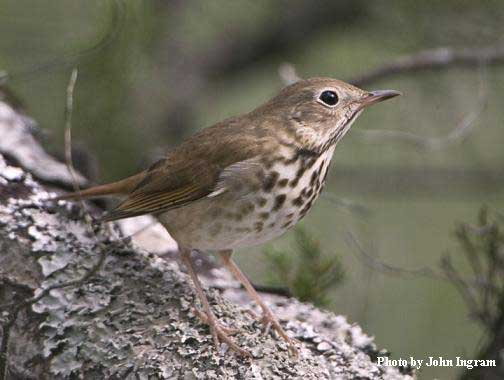
\includegraphics[width=0.65\textwidth]{figs/hermit_thrush.jpeg}
\end{center}
\column{0.5\textwidth}
\begin{center}
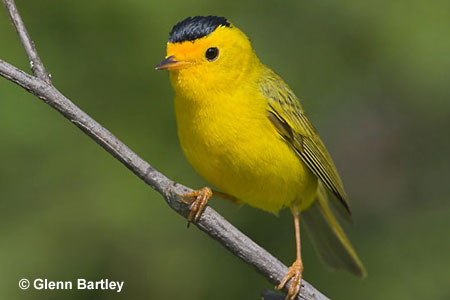
\includegraphics[width=0.65\textwidth]{figs/wilsons_warbler.jpeg}
\end{center}
\end{columns}

\end{frame}

\begin{frame}{Sampling Locations}

\begin{center}
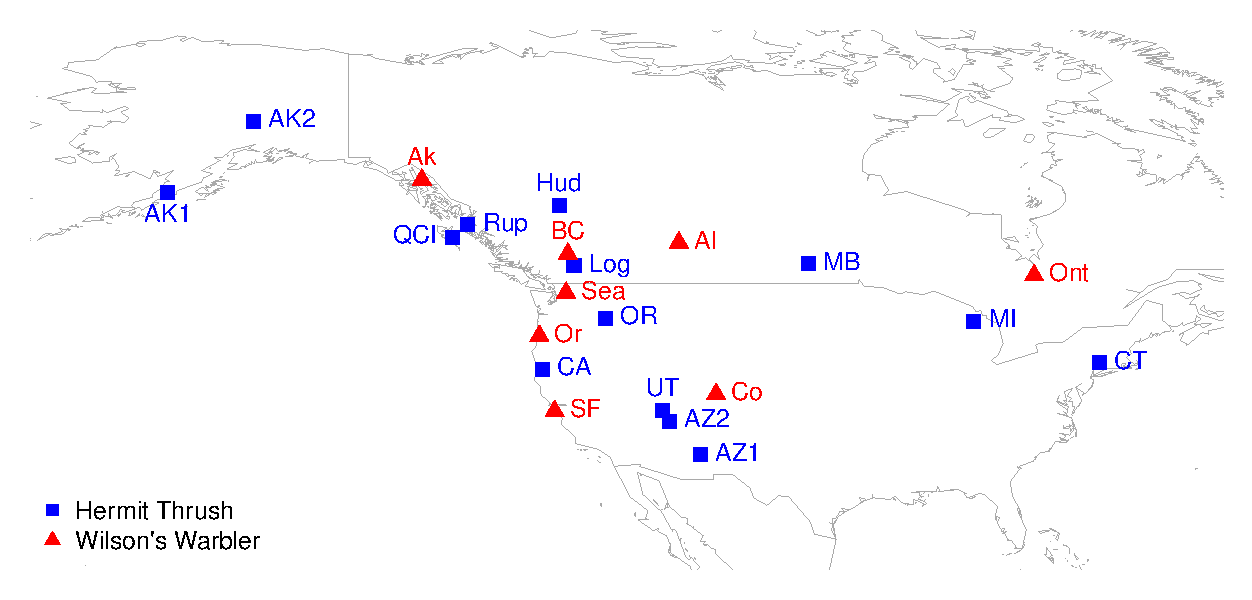
\includegraphics[width=\textwidth]{figs/sampling_locs.pdf}
\end{center}

\end{frame}

\begin{frame}{Allele Frequency Model}

For the allele \(i\), from locus \(l\), at location \(k\)

\[
\begin{aligned}
\bm{y}_{\cdot l k}|\bm{\Theta} &\sim \mathcal{N}\left(\textstyle\sum_i y_{ilk},\: \bm{f}_{\cdot l k}\right) \\
\\
f_{ilk} &= \frac{\exp(\Theta_{ilk})}{\sum_i \exp(\Theta_{ilk})} \\
\\
\bm{\Theta}_{il}|\bm{\alpha},\bm{\mu} &\sim \mathcal{N}( \bm{\mu}_{il},\, \bm{\Sigma_{}}) \\
\end{aligned}
\]

\[ \left\{\Sigma\right\}_{ij} = \sigma^2 \, \exp \Big(-(\{d\}_{ij}\, r)^{\psi} \Big) + \sigma^2_n \, {1}_{i=j} \]

\end{frame}

\begin{frame}{Predictions by Allele (Locus 3)}

\begin{center}
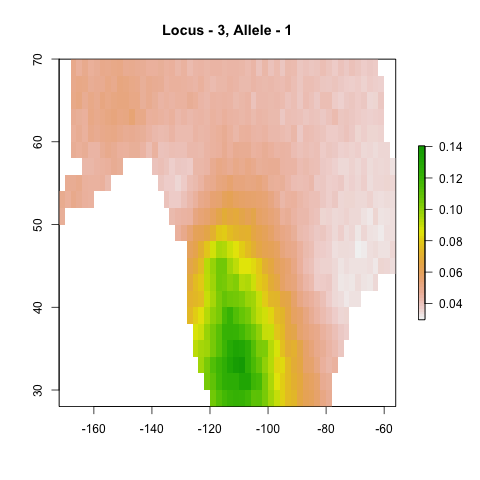
\includegraphics[width=0.25\textwidth]{figs/allele3/Med-Al3-1.png}
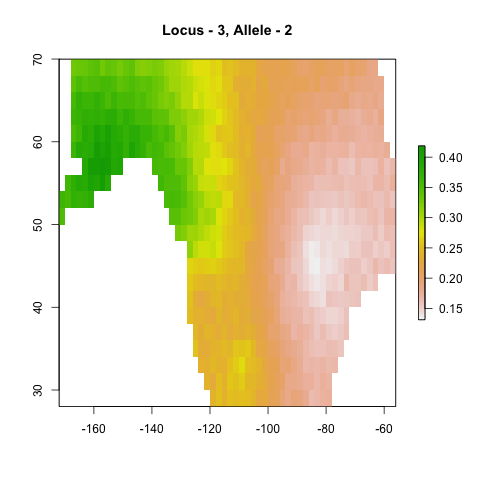
\includegraphics[width=0.25\textwidth]{figs/allele3/Med-Al3-2.png}
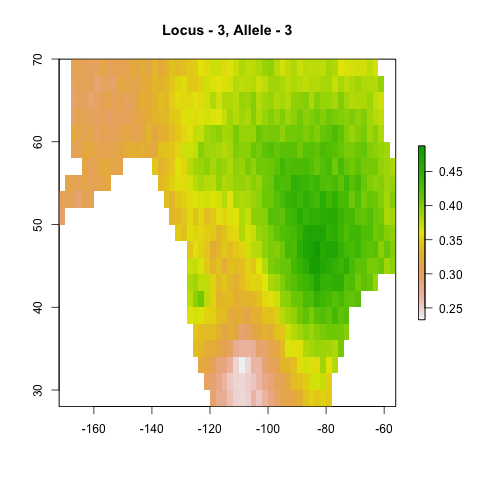
\includegraphics[width=0.25\textwidth]{figs/allele3/Med-Al3-3.png} \\
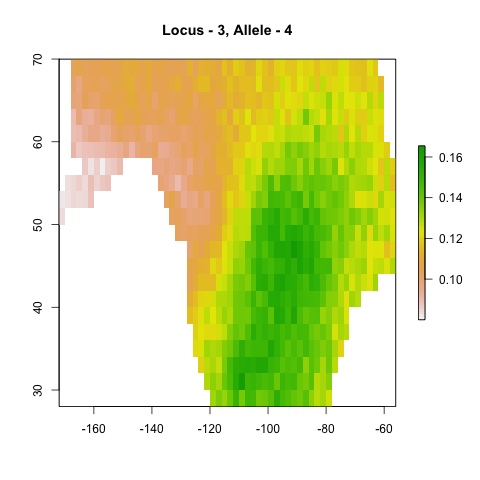
\includegraphics[width=0.25\textwidth]{figs/allele3/Med-Al3-4.png}
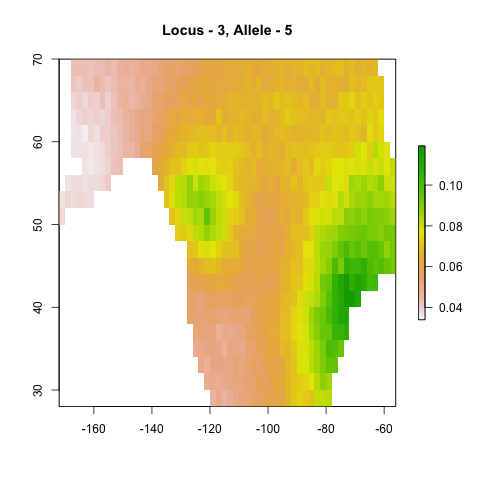
\includegraphics[width=0.25\textwidth]{figs/allele3/Med-Al3-5.png}
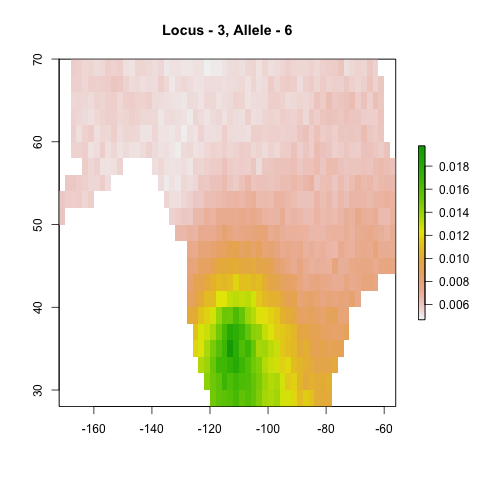
\includegraphics[width=0.25\textwidth]{figs/allele3/Med-Al3-6.png} \\
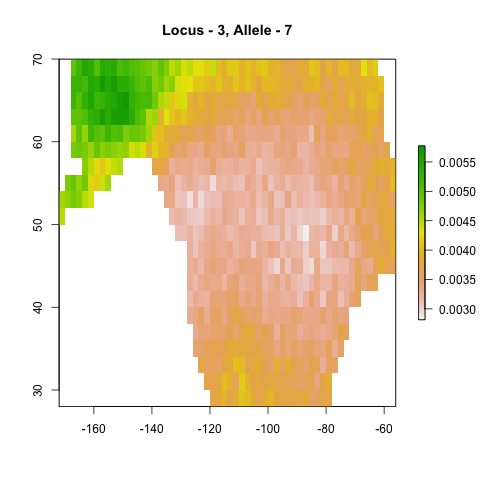
\includegraphics[width=0.25\textwidth]{figs/allele3/Med-Al3-7.png}
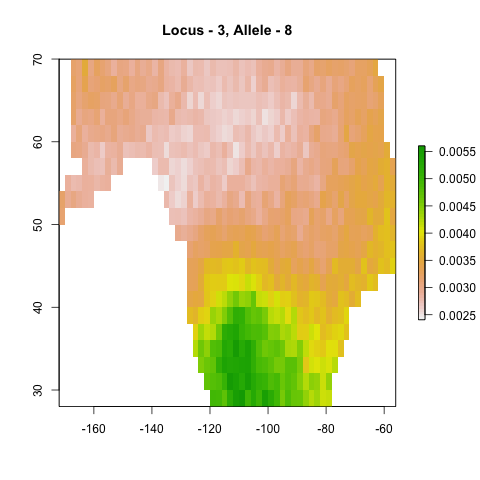
\includegraphics[width=0.25\textwidth]{figs/allele3/Med-Al3-8.png}
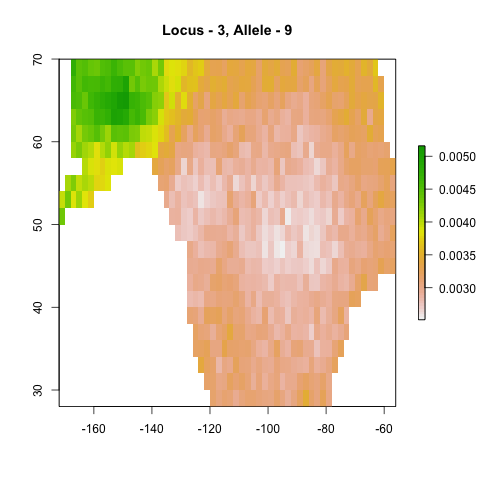
\includegraphics[width=0.25\textwidth]{figs/allele3/Med-Al3-9.png}
\end{center}

\end{frame}

\begin{frame}{Genetic Assignment Model}

Assignment model assuming Hardy-Weinberg equilibrium and allowing for
genotyping (\(\delta\)) and single amplification (\(\gamma\)) errors.

\[
\begin{aligned}
P(S_G|\bm{f},k) &= \prod_l P(i_l, j_l | \bm{f},k) \\
\\
P(i_l, j_l | \bm{f},k) &= 
\begin{cases}
\gamma P(i_l|\bm{f},k) + (1-\gamma)P(i_l|\bm{\tilde f},k)^2 & \text{if $i=j$} \vspace{2mm} \\
(1-\gamma) P(i_l|\bm{f},k) P(j_l|\bm{f},k)      & \text{if $i \ne j$}
\end{cases} \\
\\
P(i_l|\bm{f},k) &= (1-\delta) f_{lik} + \delta / m_l
\end{aligned}
\]

\end{frame}

\begin{frame}{Combined Model}

\begin{center}
Genetic \qquad\qquad\qquad\quad
Isotopic \qquad\qquad\qquad\quad
Combined
\end{center}

\begin{center}
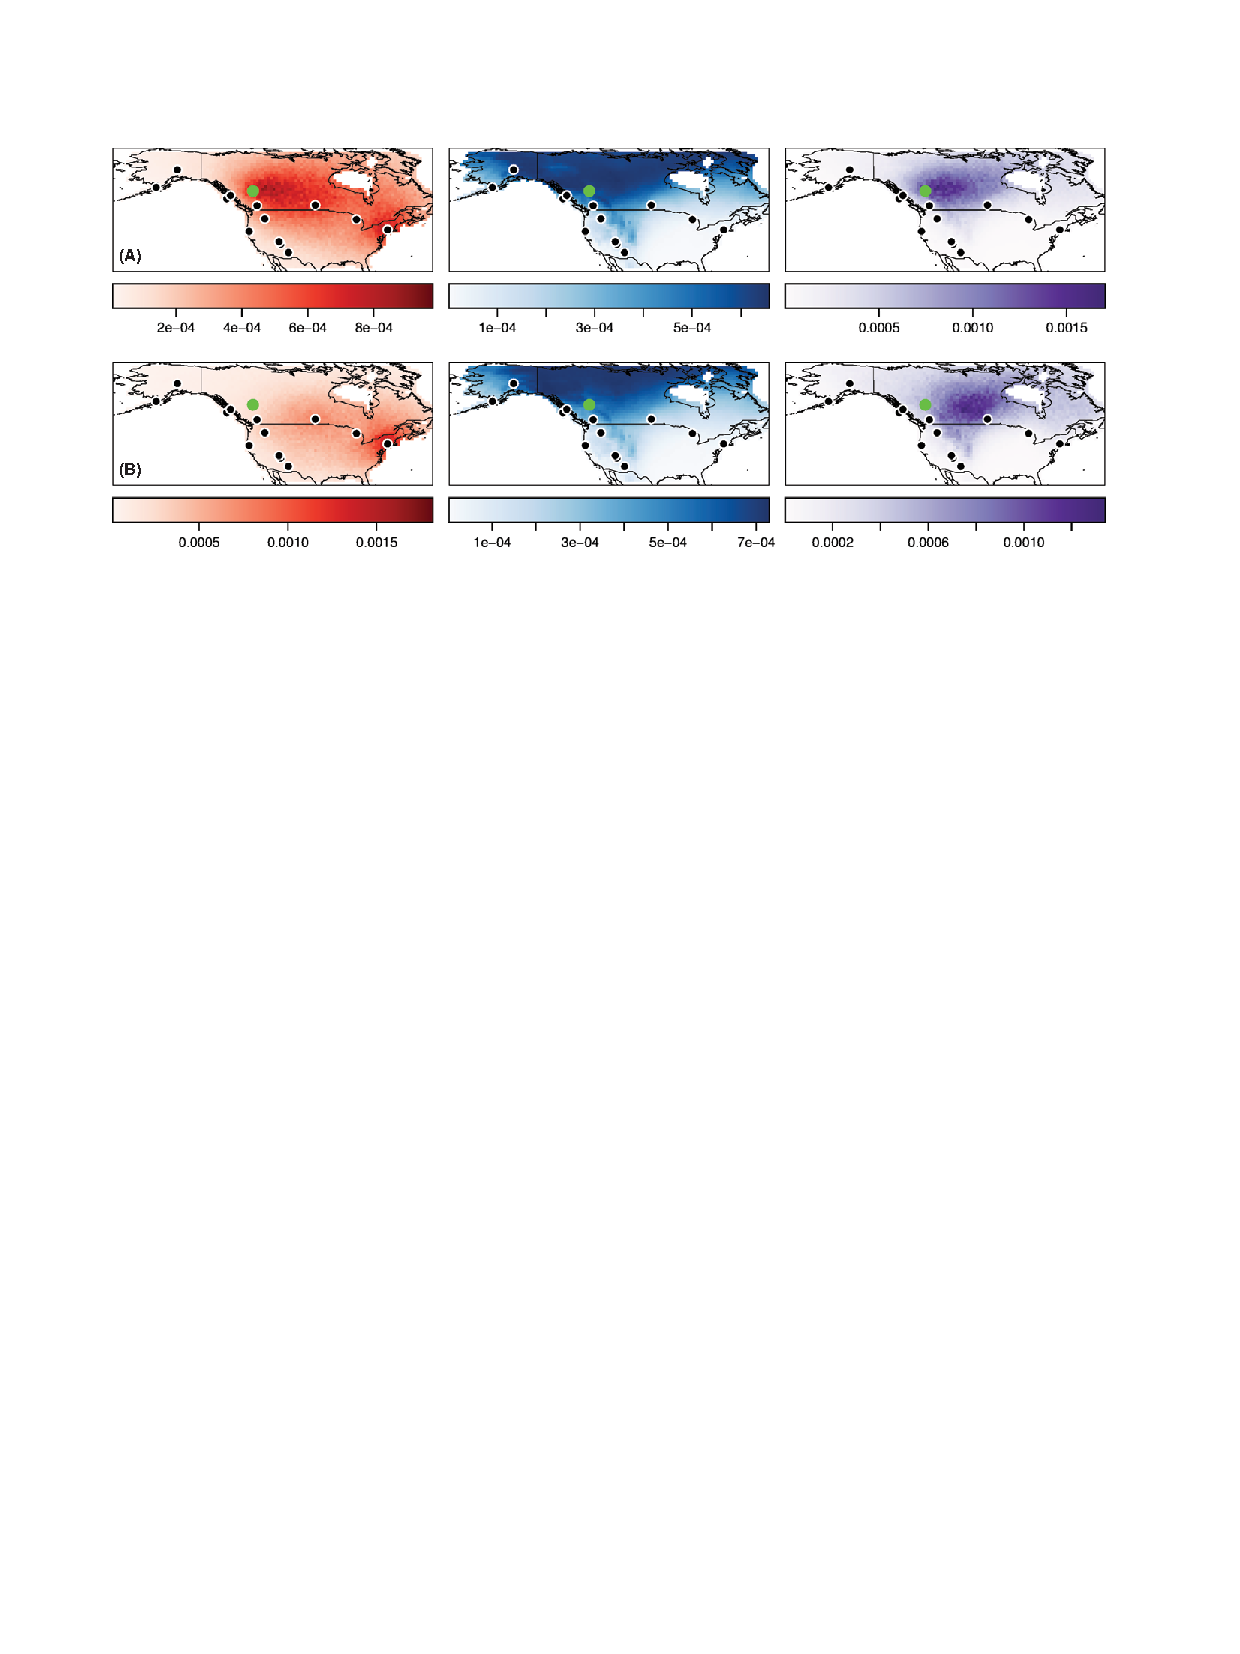
\includegraphics[width=\textwidth]{figs/hermit_maps.pdf}
\end{center}

\end{frame}

\begin{frame}{Model Assessment}

\begin{center}
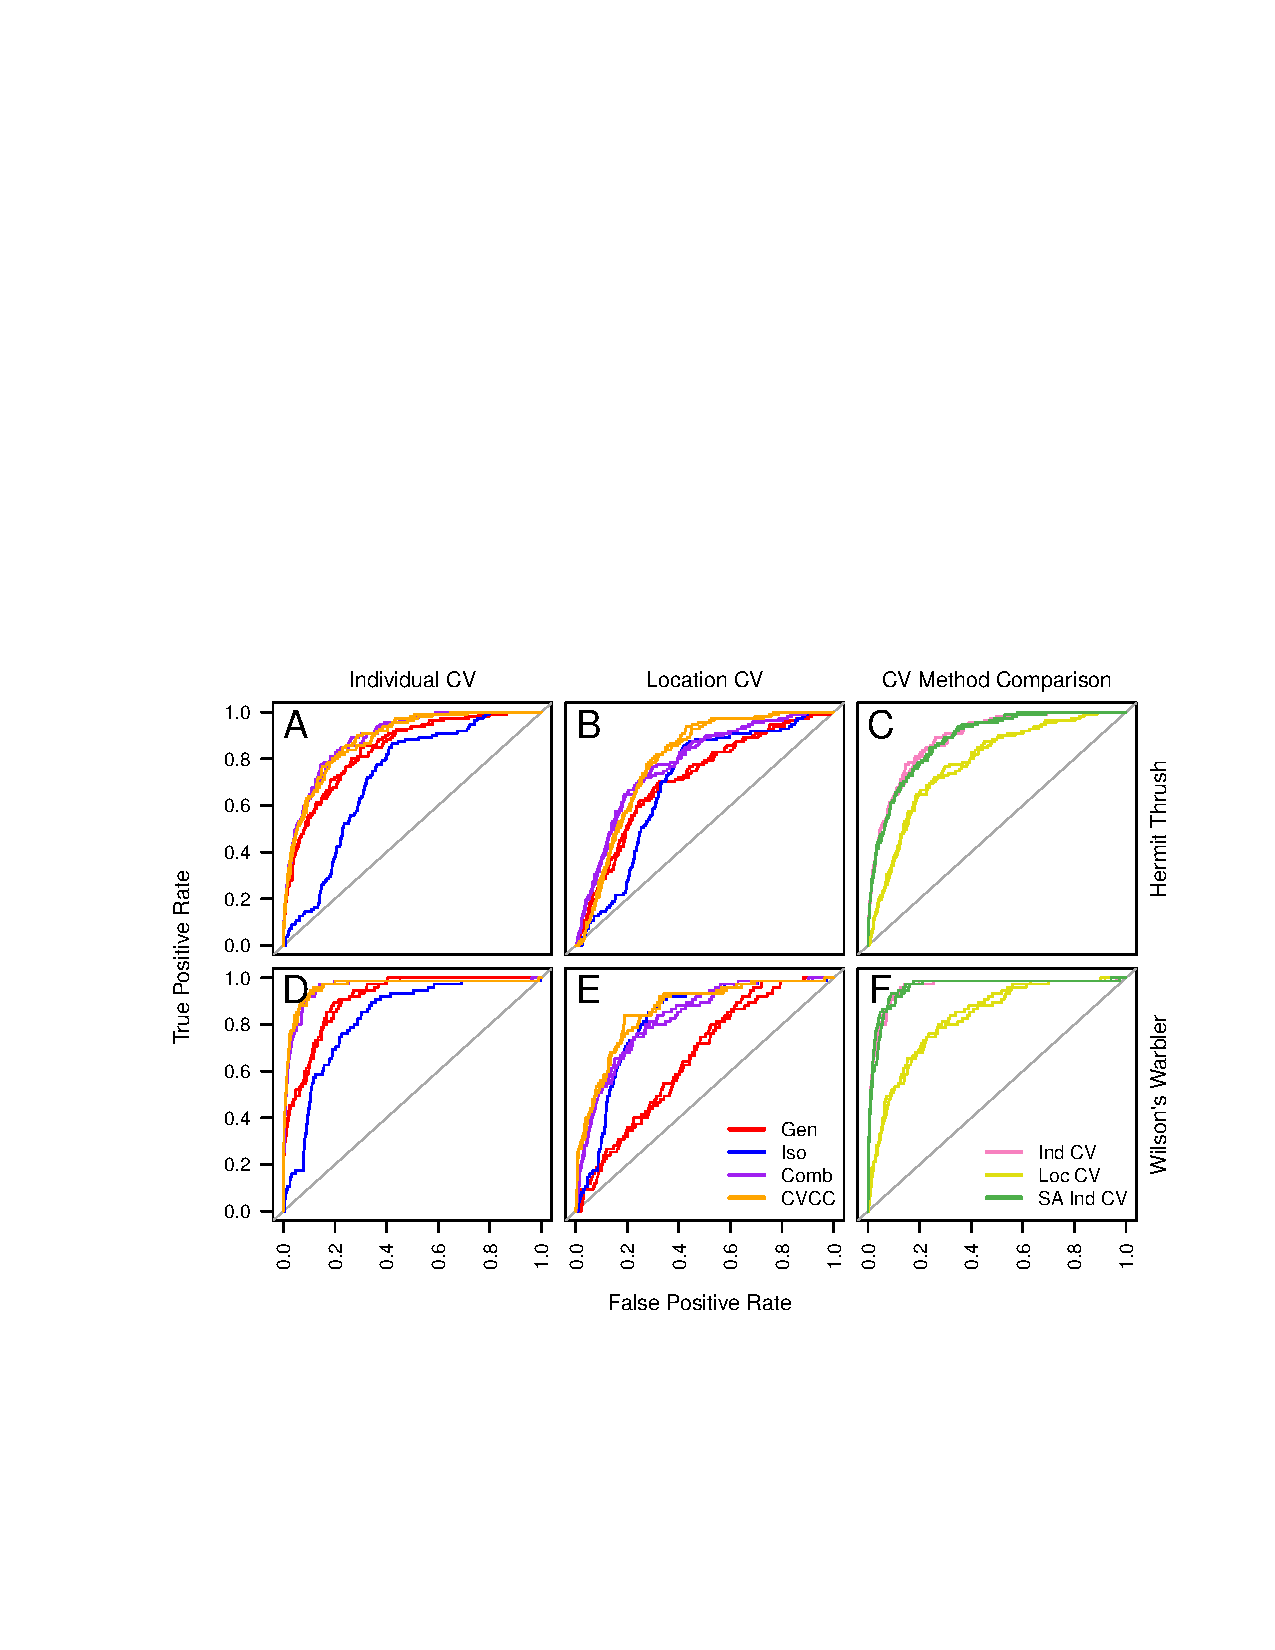
\includegraphics[width=\textwidth]{figs/ROCs.pdf}
\end{center}

\end{frame}

\begin{frame}{Migratory Connectivity}

\begin{center}
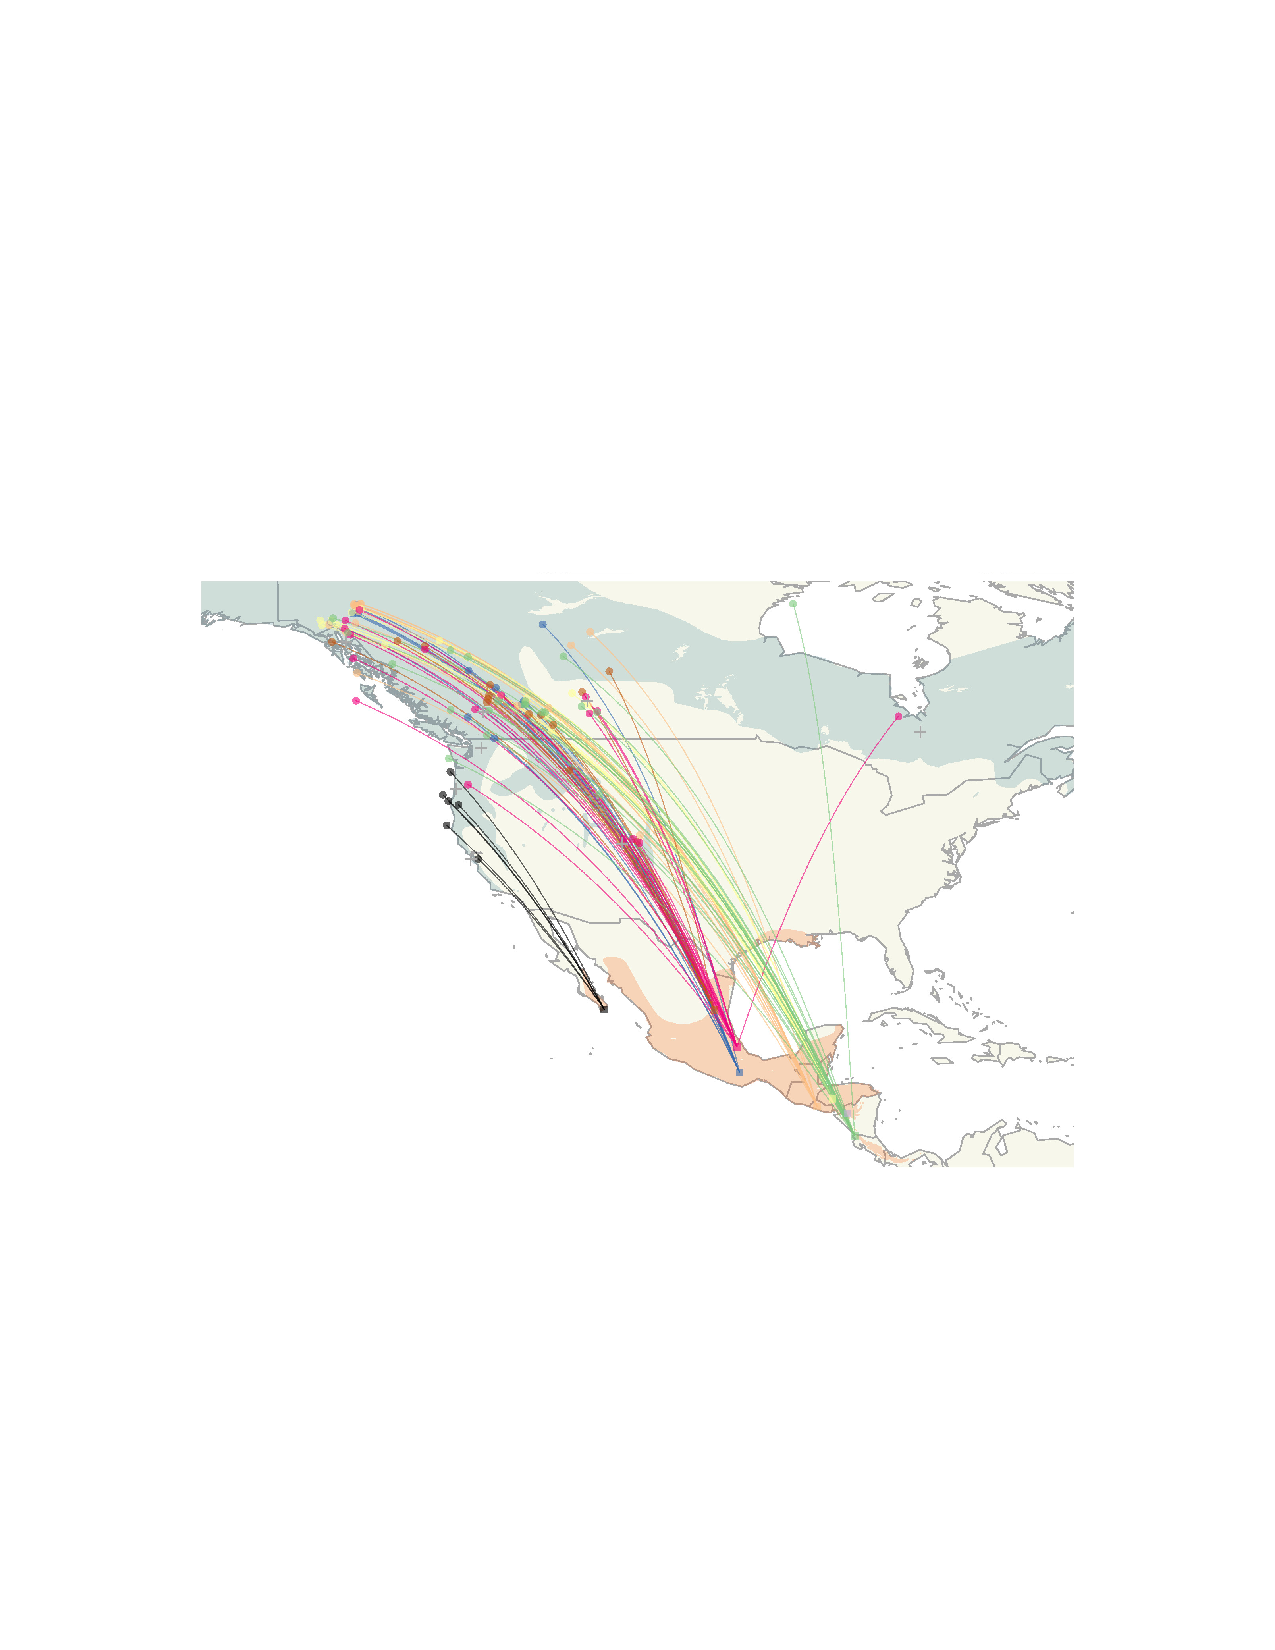
\includegraphics[width=0.9\textwidth]{figs/wintering.pdf}
\end{center}

\end{frame}

\end{document}
